\documentclass{article}
\usepackage{main}
\title{Cours : Introduction aux probabilités conditionnelles}
\author{Quentin Canu}
\date{08 Janvier 2024}

\begin{document}
\maketitle
\section{Exercice}
On lance une flèchette dans une cible : un disque séparé en 8 sections. On est assuré de toucher la cible. 
\begin{enumerate}
\item Quelle est la probabilité de toucher la section du haut ?
\item On suppose qu'on aimante les quatres sections du bas. Quelle est la probabilité de toucher la section la plus à gauche ?
\end{enumerate}
\section{Cours}
\begin{definition}
Si $A$ est un événement, alors $\overline{A}$ correspond à la non-réalisation de $A$.
\end{definition}
\begin{example}
Si $A =$ \og obtenir un $6$ au dé\fg, alors $\overline{A} =$ \og ne pas obtenir un $6$ au dé\fg.
\end{example}
\begin{definition}
Soit $A$ et $B$ deux événements. Alors $A \cap B$ correspond à la réalisation de $A$ et de $B$ en même temps.
\end{definition}
\begin{example}
Si $A =$ \og obtenir un $6$\fg et $B =$ \og obtenir un nombre pair\fg. Alors,
\begin{equation*}
P(A \cap B) = \dfrac{1}{6}\,.
\end{equation*}
\end{example}
\begin{definition}
Soit une expérience aléatoire d'univers $E$ (Exemple : le lancer d'un dé équilibré). Soit deux événement $A$ et $B$ tel que la probabilité de $B$ est non nulle. On définit la \emph{probabilité conditionnelle} de $A$ sachant que $B$ est réalisé, notée $P_B(A)$, par
\begin{equation*}
P_B(A) = \dfrac{P(A \cap B)}{P(B)}\,.
\end{equation*}
\end{definition}
\begin{example}
Avec les événements de l'exemple précédent, on obtient
\begin{equation*}
P_B(A) = \dfrac{P(A \cap B)}{P(B)} = \dfrac{\dfrac{1}{6}}{\dfrac{1}{2}} = \dfrac{1}{3}\,.
\end{equation*} 
\end{example}
Etant donné deux événements $A$ et $B$ (avec $P(B) \neq 0$), on peut construire l'arbre pondéré correspondant.
\section{Exercice}
\begin{center}
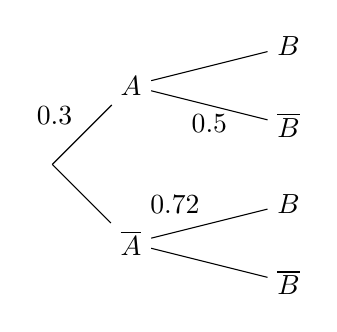
\begin{tikzpicture}
\coordinate (O) at (0,0);
\node (A) at (1,1) {$A$};
\node (Abar) at (1,-1) {$\overline{A}$};
\node (B1) at (3,1.5) {$B$};
\node (B1bar) at (3,0.5) {$\overline{B}$};
\node (B2) at (3,-0.5) {$B$};
\node (B2bar) at (3,-1.5) {$\overline{B}$};
\draw (O) -- (A) node[midway,above left] {$0.3$};
\draw (O) -- (Abar);
\draw (A) -- (B1);
\draw (A) -- (B1bar) node[midway,below] {$0.5$};
\draw (Abar) -- (B2) node[midway,above left] {$0.72$};
\draw (Abar) -- (B2bar);
\end{tikzpicture}
\end{center}
\begin{enumerate}
\item Recopier et compléter l'arbre pondéré.
\item Donner les probabilités $P(\overline{A})$, $P_A(B)$, $P_{\overline{A}}(B)$ et $P(\overline{B})$.
\end{enumerate}
\section{Exercice : SVT}
On étudie un gêne disposant de deux allèles $A$ et $a$. Un individu peut donc avoir une configuration $AA$, $Aa$ ou $aa$. Un enfant reçoit un des allèle de chacun de ses parents avec probabilité équivalente. On suppose que chacun des parents est $AA$ avec une probabilité $0.6$ et $aa$ avec une probabilité $0.1$. Le but est de dresser un arbre pondéré modélisant la situation.
\subsection*{Indications}
\begin{enumerate}
\item Combien de possibilités pour chaque parent ? Quelle est la probabilité de chacune de ces possibilités ?
\item A-t-on les mêmes possibilités pour l'enfant ? De quoi cela dépend-il ?
\item Quels événements faut-ils représenter d'abord ?
\end{enumerate}
\end{document}